\documentclass[main.tex]{subfiles}
% \nomenclature[A]{GPR}{Ground Penetrating Radar}%

\begin{document}
\chapter{Project Management}
\chaplabel{projectManagement}
\textcolor{red}{This chapter provides a high level overview of various management aspects of the project with an overview of the project goal and  any changes that occurred since the Preliminary Report. The main stakeholders involved with the project are then identified, and their roles are explained. The division of the project workload amongst the team members is shown in the work breakdown structure, and a final Gantt chart is presented to demonstrate the workload and organisation over the time-line of the project. A risk assessment is also presented and any unforeseen shortfalls discussed. Finally, the budget for the project is presented and analysed showing the funding breakdown for the project.}

Project management provides a high level overview of the management aspects of the project including the project goal and any changes that have have been made since the Preliminary Report. Division of the project workload amongst the team members is critical for completion and is determined through a work breakdown structure. A final Gantt chart was drafted to demonstrate the workload and organisation over the time-line of the project. A risk assessment was also conducted and any unforeseen shortfalls discussed as well as an analysis of the budget and expenditure for the project.

\section{Path to project completion}
% Talk about deliverables and milestones as well, taking some details from below:
%%%%%%%%%%%%%%%%%%%%%%%%%%%%%%%%%%%%%%%%
% The deliverables for the project in semester 1, 2016 are the project charter and preliminary report. These deliverables were due on 24th March and 3rd June, 2016, respectively. 
% Deliverables for semester 2, 2016 include, and is not limited to, seminar presentation, final report and  Ingenuity expo. The tentative dates for these deliverables are 20th to 22nd September, 21st October and 27th to 28th October, 2016, respectively. 
% In addition, a deliverable for a computer simulation of the platform automation and navigation is required by the date of the Ingenuity expo as this will be displayed in lieu of a platform demonstration. There are further deliverables and milestones listed in \Chapref{ganttChart} and will be modified accordingly should the need arise. 
%%%%%%%%%%%%%%%%%%%%%%%%%%%%%%%%%%%%%%%%

This project has advanced with progress swiftly and efficiently. the initial concept proposed in the project charter was to utilise a hovercraft however a change of scope was necessary to involve different land based vehicle to ensure project specifications were met. Project sponsorship through the DSTG was achieved whereby equipment loaning, technical assistance, and funding was received. The DSTG supplied the GPR, metal detector, and the quad bike as well as \$16,500 of project funds. Extensive literature reviews were completed on landmine detection methods, automation software and platform systems leading to the decisions made for the scope and direction of the project. The main project direction decided through these included the decision to use a wheeled platform with sensor fusion, where two sensory systems are used instead of one, a GPR and a metal detector. These decisions were based on research findings and through group discussions. 

With the project heavily incorporating both software and hardware system designs and development, project and team management was crucial for the timely completion of the goal and objectives. This was achieved through clear structuring of the team into required groups with each individual being assigned specific jobs and tasks within the group. Individuals were also nominated for certain systems dependent on their strengths in that field. The systems encountered throughout the project included software development for the automation of the quad bike, wireless communications, hardware modification, sensor analysis, and whole system testing.

Modifications to the Gantt chart constructed from the Preliminary report were minor due to the workload offset from the software development. A delay in platform delivery meant that advancements in software development for the automation of the platform were able to be achieved and completed ahead of schedule. Once delivery of the platform was accepted, progress was able to be achieved swiftly due to the reduced software workload allowing for more focus on the quad bike. Testing of the sensors in differing soil properties and depths allowed for comprehensive knowledge of the outputs over targets, allowing for the development of the algorithms necessary to determine the probability of whether an object is a landmine or not, and the classification of landmines.


Modifications to the detection depths highlighted in the preliminary report were necessary after sensor testing and communications with the DSTG. A maximum depth of 150mm was selected as this was the maximum testing depth used by the DSTG. Further modifications to the objectives include reducing the number of test requirements for the platform as there was limited time to incorporate all the aspects initially considered.  \textcolor{red}{other things we changed in the objectives since the prelim report}


Primary objectives that were achieved for the project can be broken down into software, platform, hardware, and sensor systems. for the platform and hardware, the objectives achieved were the modification of a platform for automation, remote operation of a platform, and the design and build of a sensor mount to adhere to the sensor requirements. For the software objectives achievements included; development of a virtual platform, wireless communication and information display in real time on a hand held device, and automation and navigation of a platform. For the sensors, the achieved objectives include algorithm development for landmine detection, reduction in false positives, landmine identification and classification, and clutter screening.

The objectives that were unable to be completed were the implementation of a physical landmine marker and the installation of a live feed camera. Emphasis was placed upon the platform automation and sensor systems and due to some delays with the communications within the last weeks before the project deadline, these objectives were unable to be fulfilled.  \textcolor{red}{oh boi}

\todo[inline]{Add something about how the project goals have changed since the beginning of the project, possible put the old goals in an appendix}

\section{Stakeholders}

The stakeholders of the project remain largely the same as in the project charter, except the DSTG is now listed as a project partner and sponsor. \Tabref{stakeholders} shows all contributing members, and describes the roles they fulfil in the project.  

\nohyphens{	% Stop hyphenation in table
\begin{longtable}{L{0.2\textwidth} L{0.25\textwidth} L{0.45\textwidth}}
\caption[Stakeholders]{Stakeholders of the project.}\tablabel{stakeholders}\\ \toprule
\textbf{Members} & \textbf{Roles} & \textbf{Description}\\ \midrule\endfirsthead 
\caption[]{Stakeholders of the project (continued).}\\ \toprule
\textbf{Members} & \textbf{Roles} & \textbf{Description}\\ \midrule\endhead

Peter Dawson & Project Manager, Document Manager & The project manager is responsible for the overall management of the project. Their tasks involve communicating with the supervisor, group members, project sponsor and other external parties. Additionally, they are responsible for assignment of tasks and chairing of meetings. The document manager is responsible for document collation and data backup. \\ \midrule

Jonathan Targett & Technical Manager & The technical manager’s responsibility is the overall management of the technical aspects of the project. The technical aspects may include procurement mechanical resources, electronic resources and other materials for the project.\\ \midrule

Rahul Kalampattel & Safety Manager & The safety manager is responsible for lloking after the safety aspects of the project. This includes conducting risk assessments, providing a safe operating procedure (SOP), overseeing the completion of such documents and liaising with the necessary third parties to provide relevant safety information.\\ \midrule

Racquel Punu & Secretary, Test Manager & The secretary is responsible for the administrative requirements of the project, including producing meeting minutes, and submission of documents through MyUni. The test manager is responsible for overall management of any testing conducted on systems and their components as required.\\ \midrule

Harrison Vince & Treasurer, Manufacturing Manager & The treasurer is responsible for managing finances within the project. The manufacturing manager is responsible for overseeing any manufacturing processes undertaken, and dealing with other design related issues.\\ \midrule

Dr Maziar Arjomandi & Project Supervisor & Supervises student members and guides them accordingly.\\ \midrule

DSTG & Project Partner and Sponsor & Supports the project and project members in providing expertise, loaning of equipment, and funding. A research agreement entitles the Project Partner to share in all knowledge gained over the course of the project.\\ \bottomrule

\end{longtable}}

Minor stakeholders include, but are not limited to, the mechanical and electrical engineering workshop staff, School of Mechanical Engineering administration staff, honours project coordinator and others as deemed necessary by the project members. Communication between all stakeholders includes, but is not limited to, email, mobile messages, phone calls, and social media. %Added because we missed it last time. 

\section{Work breakdown structure and Gantt chart}
The Work Breakdown Structure and Gantt chart were modified from the preliminary report as necessary due to the increase in project workload and objectives as the project advanced. The time line for the GPR data acquisition and software development had to be postponed due to a faulty electrical component that rendered the system inoperable. A replacement part took a long period of time to source, however, progress was not hindered by the set back. The final versions for the work breakdown structure and Gantt chart are attached in \textcolor{red}{attach the new wbs and gantt chart} 
 \Chapref{WBS,ganttChart} respectively.  
\textcolor{red}{Check that WBS is OK, go back and add more details to Gantt chart regarding deliverables such as the seminars, poster, final report}

\section{Risk management}
This section deals with the management of the various risks associated with the project. In \secref{safety}, safety risks are identified through a formal risk assessment. In \secref{risk}, risks to project failure are listed, and the consequences, controls and potential recovery methods are discussed. 

\subsection{Safety risks}
\seclabel{safety}
\textcolor{red}{Need to update this section}
Safety risks refer to those hazards that may adversely affect a person involved in the operation of the landmine detection platform. After performing a formal risk assessment (\Chapref{riskAss}), two safety risks were identified:
\begin{enumerate}
\item Risk of being caught between moving parts of a machine. This risk exists because motors and actuators are present on the quad bike, and may act as pinch points. However, the likelihood of someone interacting with the platform during operation is low, hence the residual risk is low.
\item Risk of being struck by a vehicle. This risk exists because the quad bike has the potential to behave unpredictably during testing, or become uncontrollable. Again, the likelihood of this occurring is low, and in the even that it does, controls have been put in place (emergency stop and remote kill switch). As a result, the residual risk is low.
\end{enumerate}
In order to minimise the likelihood of risks, a SOP has been developed (\Chapref{riskAss}). This document MUST be consulted before operating the quad bike. 
\nomenclature[A]{SOP}{Safe Operating Procedure}% 

\subsection{Project difficulties}% Risks of project failure}
\seclabel{risk}
\textcolor{red}{Tie this in better to the into, and the risks of project failure appendix (still need to have this as part of the assessment)}
The difficulties experienced throughout this project were numerous. they encompassed the software understanding and development required to analyse complex sensor signals to the automation and communications for the automation of the quad bike. 

Understanding of complex sensor systems and outputs as well as software development for the analysis and fusion of sensor signals was taxing and time consuming. Extensive tests and trials had to be conducted for each sensor system to be able to draw similarities between signal outputs to find the required metrics to base the detection algorithm on. These tests were time consuming and at times inconclusive requiring repeat tests to be required. One of the ongoing difficulties with the sensory systems is the changing in signal output for the GPR due to changing soil parameters. Another is the detection of composite landmines as the signals produced by them are very similar to the soils that were used for testing. \textcolor{red}{any other difficulties}

Difficulties experienced with the quad bike were associated with the communications and control of the  whole system. Issues with the communications between the ardiuno and the main computer were intermittent resulting in unsafe conditions to test the quad bike. Testing of the quad bike was also constrained to a small enclosure that limited the range of tests that could be performed on the system autonomously. To overcome these, numerous safety measures and precautions were put in place so that no damage or harm could be caused by the quad bike. Extensive bunting, barricades and a variety of kill switches and emergency stops were implemented but where never required. 
%There are a variety of reasons for which the project objectives may not be achieved; in this case, the project could be deemed a failure. The risks to project failure can be analysed by assigning each potential event with a risk level. The risk level is found by using a risk matrix, \Tabref{riskmatrix} in \Chapref{riskFailureApp}, and determining the likelihood and impact of the event. \Tabref{risks} in \Chapref{riskFailureApp} then outlines the consequences of each event, as well as the controls put in place to avoid the event, and ways to recover if the event does take place.

\section{Budget}
A number of resources were sourced and provided to support the progression of the project. They were identified as follows:
\begin{itemize}
\item School Funding: The School of Mechanical Engineering provided Honours Project students with up to \$200 per student to cover approved expenses.
\item Workshop Support: the workshop provided up to 40 hours of workshop time per student valued at \$50 per hour.
\item Supervisor time: The project supervisor contributed up to 32 hours towards the project via weekly one hour meetings.
\item Quad Bike: Through liaising with the DSTG a remotely operated quad bike was made available.
\item Detection Equipment: Through liaising with the DSTG, GPR and MD units were made available.
\end{itemize}
The final standing of the project was \$13,044.84 in credit with \$3,455.16 total expenditure. The group put 2294.5 hours towards the project totalling \$152,967 in labour costs thus far. See \secref{sponsorship}, and \secref{labourcosts} for further detail on sponsorship and labour costs, respectfully. A summary of the project expenditure can be seen in \Figref{expenditurebreakdown} with a detailed material list shown in \Chapref{budgetApp}.
\begin{figure}[ht]
\centering
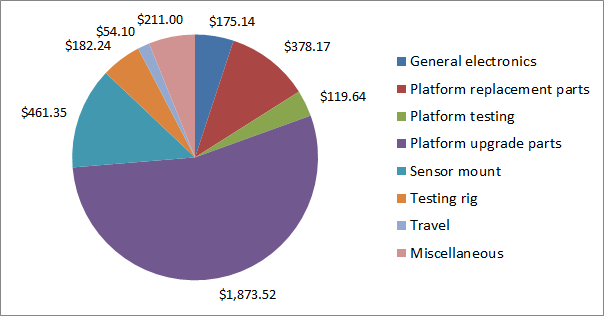
\includegraphics[]{6-ProjectManagement/expenditurebreakdown.png}
\caption[]{Expenditure breakdown}
\figlabel{expenditurebreakdown}
\end{figure}

\subsection{Sponsorship}
\seclabel{sponsorship}
It was clear from the objectives that funding would be needed to progress with the project, primarily in gaining access to expensive detection equipment and securing a mobile platform. Contact with DSTG was made and through mutual views on project outcomes, funding was granted to the value of \$16,500 as well as the supply of a remotely operated quad bike and detection equipment.

\nohyphens{	% Stop hyphenation in table
\begin{longtable}{L{0.45\textwidth} L{0.27\textwidth} L{0.18\textwidth}}
\caption{Project funding} \tablabel{funding}\\ \toprule
\textbf{Sponsor} & \textbf{Date Approved} & \textbf{Funding (\$)} \\ \midrule\endfirsthead 
\caption[]{Project Funding (continued)}\\ \toprule
\textbf{Sponsor} & \textbf{Date Approved} & \textbf{Funding (\$)} \\ \midrule\endhead
The University of Adelaide & 29/02/2016 & 1,000\\
Defence Science and Technology Group & 27/05/2016 & 16,500 \\ \midrule
\multicolumn{2}{r}{\textbf{TOTAL}} & 17,500 \\ \bottomrule 
\end{longtable}}

\subsection{Labour costs}
\seclabel{labourcosts}
To obtain a figure for the total project cost thus far, labour hours put in by each student have been tallied and included.  Each team member recorded their hourly input on a daily basis, a summarised chart is shown in \Figref{teamhours} and a detailed table can be seen in \Chapref{budgetApp}. Salaries are calculated at the rate of \$26/hr, with other direct and indirect costs included. Direct costs incur an additional 30\% on top of salary for items such as superannuation, payroll tax, workcover, long service leave, etc. Indirect costs incur an additional 130\% on top of salary for items such as administration and tech support, infrastructure, rent, phone, internet, etc. The labour costs for the project total \$152,967.
\begin{figure}[ht]
\centering
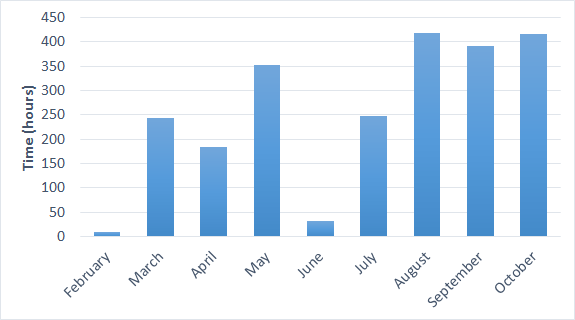
\includegraphics[]{6-ProjectManagement/teamhours.png}
\caption[]{Team hours spent on the project}
\figlabel{teamhours}
\end{figure}

\end{document}